%
% $Id: ch03_thework.tex
%
%   *******************************************************************
%   * SEE THE MAIN FILE "AllegThesis.tex" FOR MORE INFORMATION.       *
%   *******************************************************************
%
\chapter{Method of Approach} \label{ch:methods}

\name\ was developed using a modified agile approach; short development ``sprints'' were executed for key system development.
We describe the product of some of those sprints in Section~\ref{ch:methods:renderer}, primarily the ray-tracing engines.
In Section~\ref{ch:methods:interface} we also describe the Tickit interface and its algorithms.
Finally, in Section~\ref{ch:methods:threats}, we discuss drawbacks, challenges, and failures in development, as well as directions for future improvement as an open source project.


\section{Renderer Implementation} \label{ch:methods:renderer}
While building \name, two separate render engine prototypes were implemented.
The first, which we describe in Section~\ref{ch:methods:renderer:sequential}, was a simple, single core sequential renderer \cite{raytermCpuImpl}.
This engine was developed in three main development sprints, over a period of about two months.
The second, described in Section~\ref{ch:methods:renderer:parallel}, uses CUDA \cite{nvidia2011cuda} and OptiX \cite{parker2010optix} to leverage GPU compute power in parallel.
This engine was developed over two sprints, in a little under a month.


\subsection{Sequential} \label{ch:methods:renderer:sequential}

The sequential renderer, or \texttt{rayterm-cpu}, is a CPU-only ray-tracer.
It supports three different types of materials: diffuse, metallic, and dielectric.
These materials are complemented with two geometric primitives: disks, and spheres.
Figure~\ref{fig:rayterm-cpu-ppm} shows an image of the \texttt{ppm} output of \texttt{rayterm-cpu} near the end of its development.
The Tickit interface was never integrated into the CPU implementation, as this implementation is not performant enough for even simple scenes at low resolution.
For example, Figure~\ref{fig:rayterm-cpu-ppm} was rendered in about twenty seconds on a modern CPU.

\vspace{0.3em}
\begin{figure}[htb]
  \centering
  \includegraphics[width=0.75\textwidth]{impl-images/first_positionable_camera}
  \caption{\texttt{rayterm-cpu} example \texttt{ppm} output}
  \label{fig:rayterm-cpu-ppm}
\end{figure}

The main advantage of a sequential renderer is the lower development overhead, since there is no need to interface with a complex device such as a GPU.
This means that there is no need for handling parallel execution, and each ray is computed one after the other.
Because of this simplicity, this engine's development was perfectly suited the goal of gaining knowledge  and experience in ray-tracing.
The development also explored many fundamentals so that future contributions would be well-founded.
With 219 commits and over a thousand lines of code in the final product, along with many thousands of additions and deletions, \texttt{rayterm-cpu} accomplished its goals.

\littlesection{Components} \label{ch:methods:renderer:sequential:components}

The sequential renderer's implementation relies on two main components, as well as the Eigen linear algebra library \cite{eigenweb}.
These components have a linear relationship, as can be seen in Figure~\ref{fig:rayterm-cpu-components}; \texttt{raytrace} deals with tracing rays, \texttt{raymath} with intersection logic, and Eigen with linear algebra.

\vspace{0.3em}
\begin{figure}[htb]
  \centering
  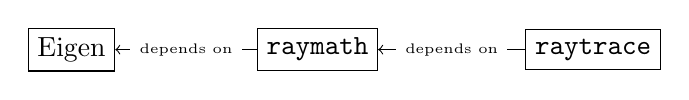
\begin{tikzpicture}
      \node[shape=rectangle,draw=black] (e) at (-3.125,0) {Eigen};
      \node[shape=rectangle,draw=black] (rm) at (0,0) {\texttt{raymath}};
      \node[shape=rectangle,draw=black] (rt) at (3.5,0) {\texttt{raytrace}};

      \path [<-](e) edge node[midway, fill=white] {\tiny depends on} (rm);
      \path [<-](rm) edge node[midway, fill=white] {\tiny depends on} (rt);
  \end{tikzpicture}
  \caption{Component and dependency relationships in \texttt{rayterm-cpu}}
  \label{fig:rayterm-cpu-components}
\end{figure}

Eigen \cite{eigenweb} is a linear algebra for C++ that supports matrix and vector manupulations, various matrix decompositions and geometry features, and has many extensions for numerous other numerical operations.
Eigen is also extremely well-optimized and uses SSE vectorized code, vastly improving performance on supported CPUs.
In \texttt{raymath}, Eigen is used primarily for easy, tested representations and calculations involving vectors; all of the algorithms implemented use equations derived from the ones in Section~\ref{ch:intro:background:raytracing_math}, and so benefit from easy implementation.

The base component in \texttt{rayterm-cpu} -- \texttt{raymath} -- provides support for various geometries and intersection routines. The geometries supported can be seen in Figure~\ref{fig:rayterm-cpu-raymath-geometry}, and use Eigen structures to represent their geometric data.
\texttt{raymath} also handles random number and vector generation, color handling, and intersection representation.
The implementations behind these are covered in Section~\ref{ch:implementation:rayterm-cpu:raymath}.

\vspace{0.3em}
\begin{figure}[htb]
  \centering
  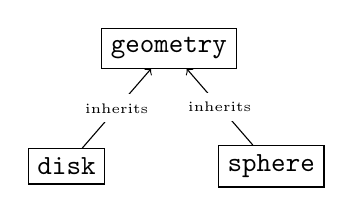
\begin{tikzpicture}
    \node[shape=rectangle,draw=black] (g) at (0,1.5) {\texttt{geometry}};
      \node[shape=rectangle,draw=black] (s) at (1.3,0) {\texttt{sphere}};
      \node[shape=rectangle,draw=black] (d) at (-1.3,0) {\texttt{disk}};

      \path [<-](g) edge node[midway, fill=white] {\tiny inherits} (s);
      \path [<-](g) edge node[midway, fill=white] {\tiny inherits} (d);
  \end{tikzpicture}
  \caption{Geometric structures in \texttt{raymath}}
  \label{fig:rayterm-cpu-raymath-geometry}
\end{figure}

The main component in \texttt{rayterm-cpu} is \texttt{raytrace}; it handles world representation, materials, and raytracing.
\texttt{rayterm-cpu} only renders in \texttt{ppm} mode, since the Tickit interface was only integrated in the \texttt{rayterm-gpu} implementation, since that was the final prototype.
\texttt{raytrace} represents objects with a \texttt{WorldObject} class, a list of which is stored in a \texttt{World}.

Figure~\ref{fig:rayterm-cpu-raytrace-journey-of-a-ray} shows the function call path that is used when rendering a single ray.
The main entry point is \texttt{raytrace\_ppm}, which creates rays with a \texttt{Camera} class instance.
This instance contains specific parameters to control the position and orientation of the virtual camera, and thus controls where the \texttt{ray} originates from. and its direction.
Then, that \texttt{ray} is sent on to the \texttt{World} class, where an \texttt{intersection} is retrieved, and then used to generate a \texttt{color} from the given \texttt{ray}.
This color is then finally returned to \texttt{raytrace\_ppm}, which writes it to a \texttt{ppm} file.
Unmentioned in this diagram are the recursive calls to \texttt{World::trace} from from \texttt{WorldObject::colorize}, which use the transformed ``scatter'' \texttt{ray} from \texttt{Material::scatter}.
The implementation behind all of these structures and functions are covered in Section~\ref{ch:implementation:rayterm-cpu:raytrace}.

\vspace{0.3em}
\begin{figure}[htb]
  \centering
  \begin{tikzpicture}
    \node[shape=rectangle, draw=black] (a) at (0,0) {Ray collection in \texttt{raytrace\_ppm}};
    \node[shape=rectangle, draw=black, right = 2.5em of a ] (b) {Generation in \texttt{Camera::get\_screen\_ray}};
    \node[shape=rectangle, draw=black, below = 1.75em of a] (c) {World tracing in \texttt{World::trace}};
    \node[shape=rectangle, draw=black, right = 2.5em of c] (e) {Ray coloring in \texttt{WorldObject::colorize}};
    \node[shape=rectangle, draw=black, below = 1.75em of e] (s) {Ray scattering in \texttt{Material::scatter}};
    \node[shape=rectangle, draw=black, below = 1.75em of c] (d) {World intersection in \texttt{World::intersects}};
    \begin{scope}[xshift=1cm]
      \node[shape=rectangle, draw=black] (f) at (2.75, -4.15) {Object intersection in \texttt{WorldObject::intersects}};
      \node[shape=rectangle, draw=black, below = 1.75em of f] (g) {Geometry intersection in \texttt{geometry::intersects}};
      \path [->](d) edge node[midway, fill=white] {\tiny calls} (f);
      \path [->](f) edge node[midway, fill=white] {\tiny calls} (g);
    \end{scope}

      \path [->](a) edge node[midway, fill=white] {\tiny calls} (b);
      \path [->](a) edge node[midway, fill=white] {\tiny calls} (c);
      \path [->](c) edge node[midway, fill=white] {\tiny calls} (d);
      \path [->](c) edge node[midway, fill=white] {\tiny calls} (e);
      \path [->](e) edge node[midway, fill=white] {\tiny calls} (s);
  \end{tikzpicture}
  \caption{The journey of a \texttt{ray} and its \texttt{intersection}}
  \label{fig:rayterm-cpu-raytrace-journey-of-a-ray}
\end{figure}

\littlesection{Algorithms} \label{ch:methods:renderer:sequential:algorithms}

The sequential renderer implements single-branch Monte Carlo ray-tracing, a type of rendering that can produce physically accurate images with little development effort.
The algorithm is largely based on randomness, only modifying the path of a single ray as it bounces around the scene.
When encountering objects, a particular Probability Distribution Function (PDF) is used to calculate where the ray will bounce.
These PDFs vary based on the material, and are hardcoded in the \texttt{Material} implementation.
The result of this algorithm is extremely noisy because of this randomness (see Figure~\ref{fig:rayterm-cpu-ppm-noisy}), so many samples must be taken and then averaged to gain a true value for a single pixel; this simulates the many millions of photons that would have traveled to that pixel in a real camera.
The number of samples per pixel, sometimes termed ``spp,'' is the number of rays generated from a random origin within the pixel.
An example of various spp values is shown in Figure~\ref{fig:rayterm-cpu-ppm-noisy}.

\vspace{0.3em}
\begin{figure}[htb]
  \centering
  \begin{subfigure}[htb]{0.45\textwidth}
    \includegraphics[width=\textwidth]{impl-images/comparisons/samples_spp_1}
    \caption{1 sample per pixel}
    \label{fig:rayterm-cpu-ppm-noisy-1}
  \end{subfigure}
  \hspace{1em}
  \begin{subfigure}[htb]{0.45\textwidth}
    \includegraphics[width=\textwidth]{impl-images/comparisons/samples_spp_4}
    \caption{4 samples per pixel}
    \label{fig:rayterm-cpu-ppm-noisy-4}
  \end{subfigure}
  \vspace{1em}
  \begin{subfigure}[htb]{0.45\textwidth}
    \includegraphics[width=\textwidth]{impl-images/comparisons/samples_spp_32}
    \caption{32 samples per pixel}
    \label{fig:rayterm-cpu-ppm-noisy-32}
  \end{subfigure}
  \hspace{1em}
  \begin{subfigure}[htb]{0.45\textwidth}
    \includegraphics[width=\textwidth]{impl-images/comparisons/samples_spp_1024}
    \caption{1024 samples per pixel}
    \label{fig:rayterm-cpu-ppm-noisy-1024}
  \end{subfigure}
  \caption{Sample per pixel differentiated output from \texttt{rayterm-cpu}}
  \label{fig:rayterm-cpu-ppm-noisy}
\end{figure}

\littlesection{Prototype} \label{ch:methods:renderer:sequential:prototype}

This section describes the lessons learned from CPU implementation, and how the GPU implementation will differ and improve because of this step.

The final implementation of \texttt{rayterm-cpu} only renders images through a Google Test \cite{googletest} case, which can be run with the \texttt{test.sh} script in the implementation repository \cite{raytermCpuImpl}, or \texttt{gradle test}.
This generates a \texttt{test\_image.ppm} file, examples of which we show from various stages of development in Section~\ref{ch:implementation:rayterm-cpu:raytrace}.
Because of this, \texttt{rayterm-cpu} is very much a proof-of-concept and learning example, rather than a fully-fledged library.

\subsection{Parallel} \label{ch:methods:renderer:parallel}

After the implementation of \texttt{rayterm-cpu}, more performance was needed for the final \name\ implementation.
The solution to this problem was to use a Graphics Processing Unit (GPU) to drastically parallellize the raytracing algorithm.
This improves performance dramatically, because each eye-ray's children (the result of a collision between an object and a ray) are dependant on only their parent eye-ray.
Thus, the computation of a single pixel's color is completely independent of every other pixel.

A short introduction to GPUs may be useful here; they consist primarily of small units of computation circuitry called ``multiprocessors'' which themselves are controllers for several CUDA cores \cite{fermi2009nvidia}, distributing workloads.
These CUDA cores execute individual threads on the GPU, and act somewhat like advanced floating point arithmatic computation units.
A discussion on the specific hardware used for development and testing is available in Section~\ref{ch:intro:background:hardware}.

With 227 commits and over 1.5 thousand lines of code, along with many thousands of additions and deletions, \texttt{rayterm-gpu} has a good start on its life.
There are many, many more improvements possible, however.
We detail some of them in the context of the larger \name\ implementation in Section~\ref{ch:methods:threats}.

\littlesection{Libraries} \label{ch:methods:renderer:parallel:libraries}

This section talks about OptiX and CUDA.

\littlesection{Design} \label{ch:methods:renderer:parallel:design}

This section is about the code structure and organization in the \texttt{rayterm} implementation.

\littlesection{Demonstration} \label{ch:methods:renderer:parallel:demo}

This is a demonstration section on final renderer is capabable of -- this section uses only \texttt{ppm} output.

\section{Interface Implementation} \label{ch:methods:interface}

\subsection{Design} \label{ch:methods:interface:design}
